\documentclass[tikz,border=10pt]{standalone}
\usepackage{amsmath}
\usetikzlibrary{arrows.meta,positioning,backgrounds,patterns}
\begin{document}
% Shared chapter style: white canvas, sans-serif text, 0.9 pt strokes,
% restrained rounded process boxes, and 3 mm Latex arrowheads.
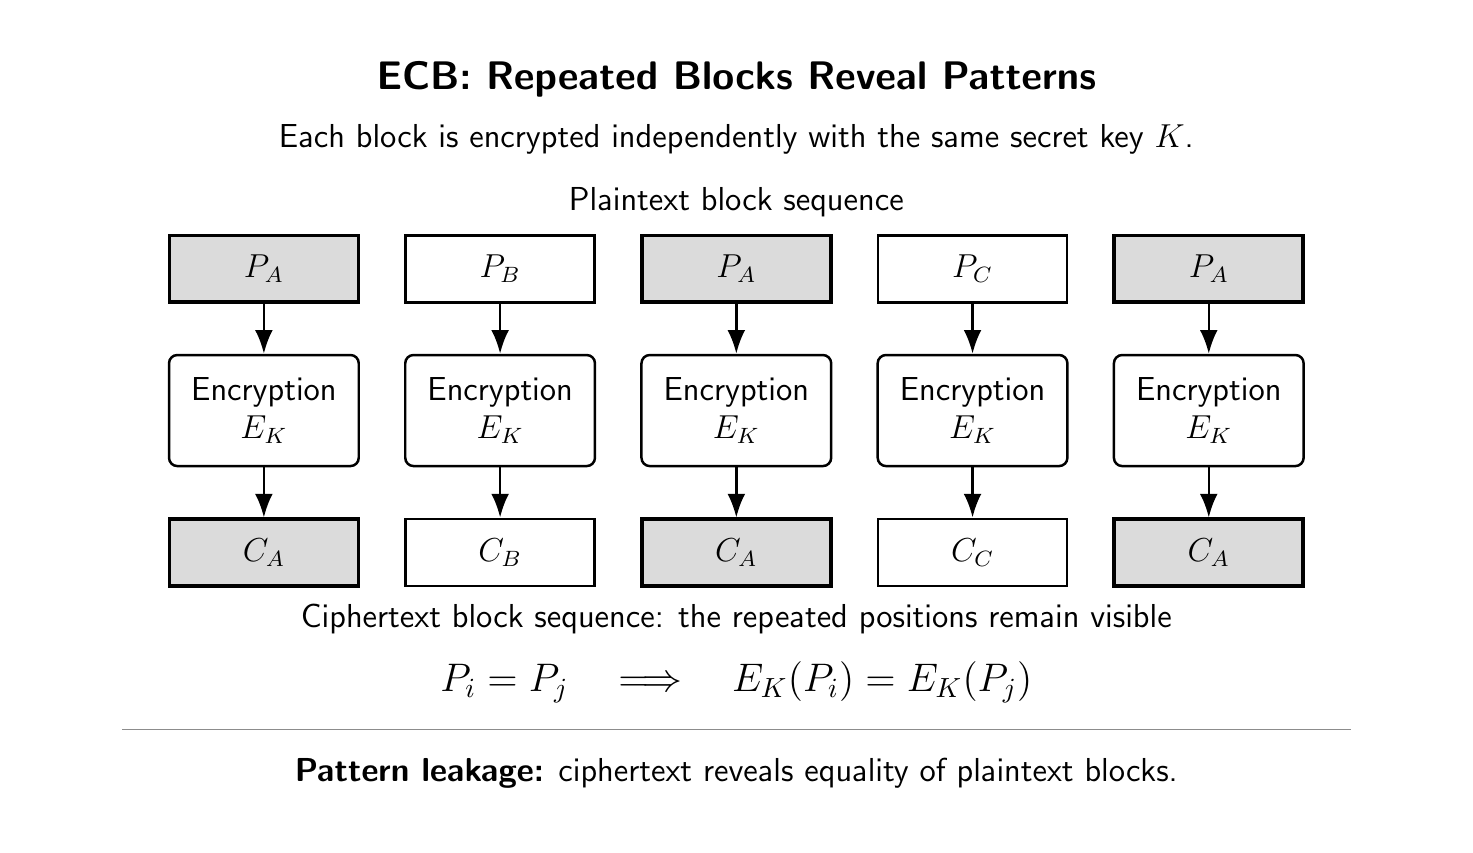
\begin{tikzpicture}[
    font=\sffamily\large, line width=0.9pt,
    background rectangle/.style={fill=white,draw=none},
    show background rectangle,
    box/.style={draw,fill=white,rounded corners=3pt,align=center,inner sep=8pt},
    data/.style={draw,fill=white,align=center,minimum width=2.4cm,minimum height=0.85cm},
    enc/.style={box,minimum width=2.4cm,minimum height=1.05cm},
    arrow/.style={-{Latex[length=3mm]},line width=0.9pt},
    title/.style={font=\sffamily\Large\bfseries,align=center},
    note/.style={align=center},
    repeated/.style={fill=black!14,line width=1.3pt}
]
\path[use as bounding box] (-9,-5.0625) rectangle (9,5.0625);

\node[title] at (0,4.4) {ECB: Repeated Blocks Reveal Patterns};
\node[note] at (0,3.65) {Each block is encrypted independently with the same secret key $K$.};
\node[note] at (0,2.85) {Plaintext block sequence};
\foreach \x/\i/\v in {-6/1/A,-3/2/B,0/3/A,3/4/C,6/5/A} {
    \node[data] (p\i) at (\x,2) {$P_{\v}$};
    \node[enc] (e\i) at (\x,0.2) {Encryption\\$E_K$};
    \node[data] (c\i) at (\x,-1.6) {$C_{\v}$};
    \draw[arrow] (p\i.south) -- (e\i.north);
    \draw[arrow] (e\i.south) -- (c\i.north);
}
% Identical visual treatment above and below makes equality visible in print.
\foreach \x/\i in {-6/1,0/3,6/5} {
    \node[data,repeated] at (\x,2) {$P_A$};
    \node[data,repeated] at (\x,-1.6) {$C_A$};
}
\node[note] at (0,-2.45) {Ciphertext block sequence: the repeated positions remain visible};
\node[font=\sffamily\Large] at (0,-3.25)
    {$P_i=P_j\quad\Longrightarrow\quad E_K(P_i)=E_K(P_j)$};
\draw[black!45,line width=0.6pt] (-7.8,-3.85) -- (7.8,-3.85);
\node[note] at (0,-4.4)
    {\textbf{Pattern leakage:} ciphertext reveals equality of plaintext blocks.};
\end{tikzpicture}
\end{document}
